\begin{figure}[H]
  \centering
  \pgfplotsset{
    scaled y ticks=false,
    scale only axis,
    legend style={at={(0,0.8)}, anchor=west, font=\tiny},
    xmin=7,
  }
  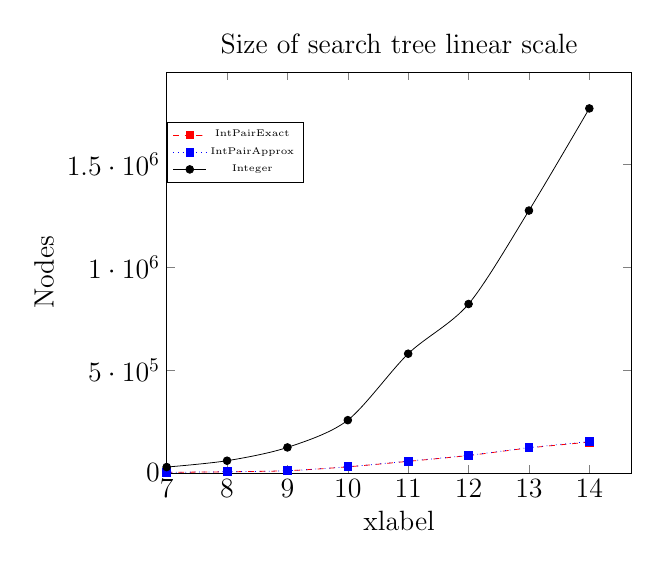
\begin{tikzpicture} [scale=0.7, font=\Large]
    \begin{axis}[
        title=Size of search tree linear scale,
        ylabel=Nodes,
        xtick=data,
        ymin=0, 
        xlabel=xlabel ]
      \addplot[smooth,mark=square*, mark options={solid},red, dashed]
      coordinates{ (7,2958) (8,5736) (9,10828) (10,29788) (11,56360) (12,84790) (13,121412) (14,149710)
      }; \label{ie_plot} \addlegendentry{IntPairExact}
      \addplot[smooth,mark=square*, mark options={solid},blue, dotted]
      coordinates{ (7,3048) (8,5862) (9,11196) (10,30142) (11,57388) (12,85692) (13,122932) (14,152074)
      }; \label{ia_plot} \addlegendentry{IntPairApprox}
      \addplot[smooth,mark=*,mark options={solid},black]
      coordinates{ (7,28628) (8,59430) (9,123970) (10,256300) (11,578818) (12,820070) (13,1273624) (14,1769398)
      }; \label{int_plot} \addlegendentry{Integer}
    \end{axis}
  \end{tikzpicture}
  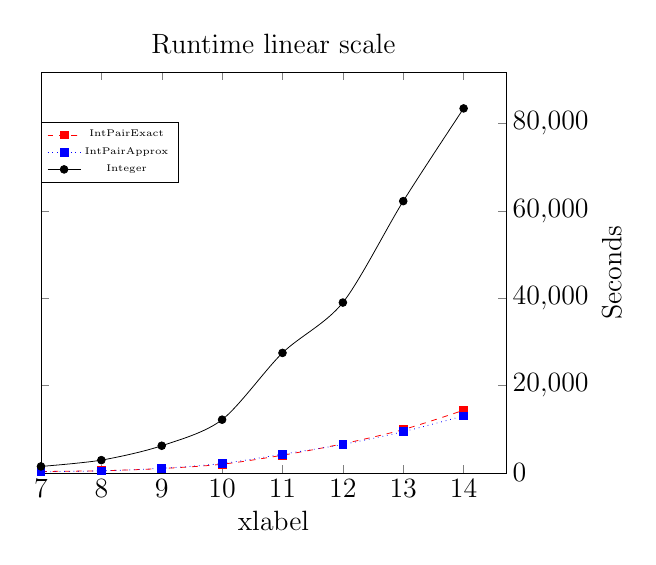
\begin{tikzpicture} [scale=0.7, font=\Large]
    \begin{axis}[
        yticklabel pos=right,
        xtick=data,
        title=Runtime linear scale,
        ylabel=Seconds,
        xlabel=xlabel,
        ymin=0, ]
      \addplot[smooth,mark=square*,mark options={solid},red, dashed]
      coordinates{ (7, 334) (8, 510) (9, 1013) (10, 2003) (11, 4064) (12, 6674) (13, 9931) (14, 14352)
      }; \label{IntPairExact Run}
      \addplot[smooth,mark=square*,mark options={solid},blue, dotted]
      coordinates{ (7, 280) (8, 483) (9, 1058) (10, 2176) (11, 4301) (12, 6529) (13, 9458) (14, 13055)
      }; \label{IntPairApprox Run}
      \addplot[smooth,mark=*,mark options={solid},black]
      coordinates{ (7, 1496) (8, 2939) (9, 6230) (10, 12194) (11, 27479) (12, 39001) (13, 62211) (14, 83431)
      }; \label{IntegerRun}
      \addlegendentry{IntPairExact}
      \addlegendentry{IntPairApprox}
      \addlegendentry{Integer}
    \end{axis}
  \end{tikzpicture}

  
\begin{tikzpicture}[scale=1.4]
    \draw[very thick] (-4,0) -- (4,0);
    \draw[draw=white] (-5,-0.2) -- (5,-0.2);
  \end{tikzpicture}


  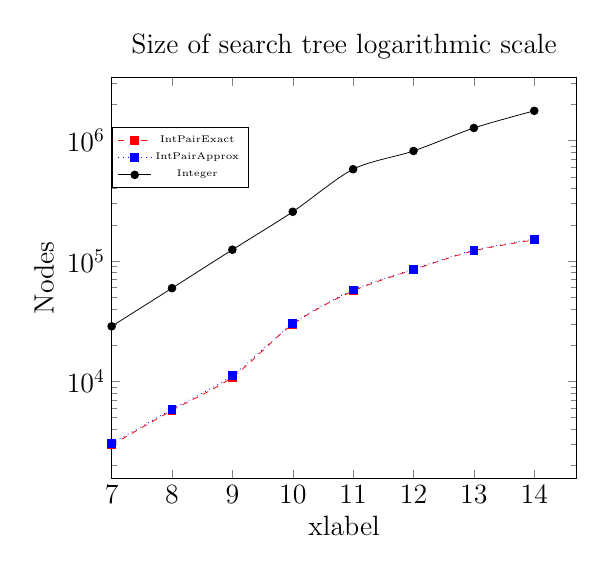
\begin{tikzpicture} [scale=0.7, font=\Large]
    \begin{semilogyaxis}[
        title=Size of search tree logarithmic scale,
        ylabel=Nodes,
        xtick=data,
        ymin=0, 
        xlabel=xlabel ]
     \addplot[smooth,mark=square*, mark options={solid},red, dashed]
      coordinates{ (7,2958) (8,5736) (9,10828) (10,29788) (11,56360) (12,84790) (13,121412) (14,149710)
      }; \label{ie_plot} \addlegendentry{IntPairExact}
      \addplot[smooth,mark=square*, mark options={solid},blue, dotted]
      coordinates{ (7,3048) (8,5862) (9,11196) (10,30142) (11,57388) (12,85692) (13,122932) (14,152074)
      }; \label{ia_plot} \addlegendentry{IntPairApprox}
      \addplot[smooth,mark=*,mark options={solid},black]
      coordinates{ (7,28628) (8,59430) (9,123970) (10,256300) (11,578818) (12,820070) (13,1273624) (14,1769398)
      }; \label{int_plot} \addlegendentry{Integer}

    \end{semilogyaxis}
  \end{tikzpicture}
  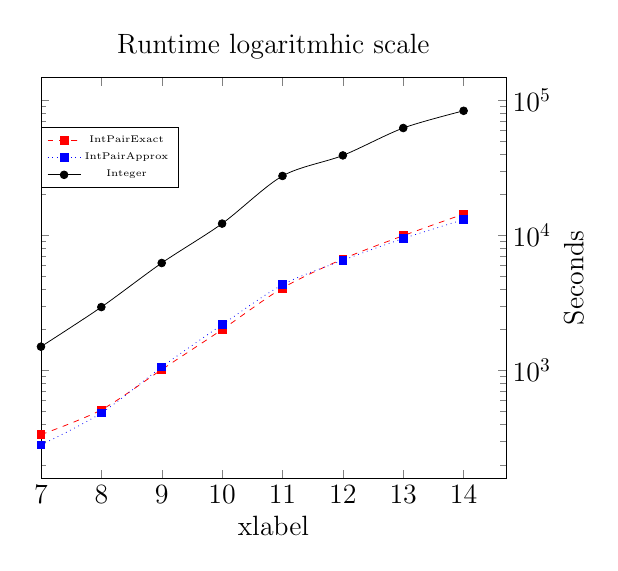
\begin{tikzpicture} [scale=0.7, font=\Large]
    \begin{semilogyaxis}[
        title=Runtime logaritmhic scale,
        yticklabel pos=right,
        xtick=data,
        ylabel=Seconds,
        xlabel=xlabel,
        ymin=0,  ]
      \addplot[smooth,mark=square*,mark options={solid},red, dashed]
      coordinates{ (7, 334) (8, 510) (9, 1013) (10, 2003) (11, 4064) (12, 6674) (13, 9931) (14, 14352)
      }; \label{IntPairExact Run}
      \addplot[smooth,mark=square*,mark options={solid},blue, dotted]
      coordinates{ (7, 280) (8, 483) (9, 1058) (10, 2176) (11, 4301) (12, 6529) (13, 9458) (14, 13055)
      }; \label{IntPairApprox Run}
      \addplot[smooth,mark=*,mark options={solid},black]
      coordinates{ (7, 1496) (8, 2939) (9, 6230) (10, 12194) (11, 27479) (12, 39001) (13, 62211) (14, 83431)
      }; \label{IntegerRun}
      \addlegendentry{IntPairExact}
      \addlegendentry{IntPairApprox}
      \addlegendentry{Integer}
    \end{semilogyaxis}
  \end{tikzpicture}
%  \input{}
%\end{figure}
  \caption{Varying the number of symbols. The other parameters are fixed: number of states=7, max cost per transition=15, and number of steps=7.}\label{fig:symbols}
 \end{figure}
